\documentclass[11pt]{article}
%Gummi|065|=)
\title{\textbf{Meccano heptagons}}
\author{https://github.com/heptagons/meccano/hepta}
\date{}

\usepackage{amsmath}
\usepackage[pdftex]{graphicx}
\usepackage{listings}
\usepackage{xcolor}
\definecolor{gray}{RGB}{245,245,245}
\usepackage{hyperref}

\lstset{
	backgroundcolor=\color{gray},
	frame=single,
	language=c,
	numbers=left,
	stepnumber=1
}

\usepackage[margin=0.75in]{geometry}

% inkscape fig.svg --export-pdf=fig.pdf (prior version 1.0)

\usepackage{graphicx}
\begin{document}

\maketitle

\section{Meccano heptagons}

\begin{figure}[htp]
\centering
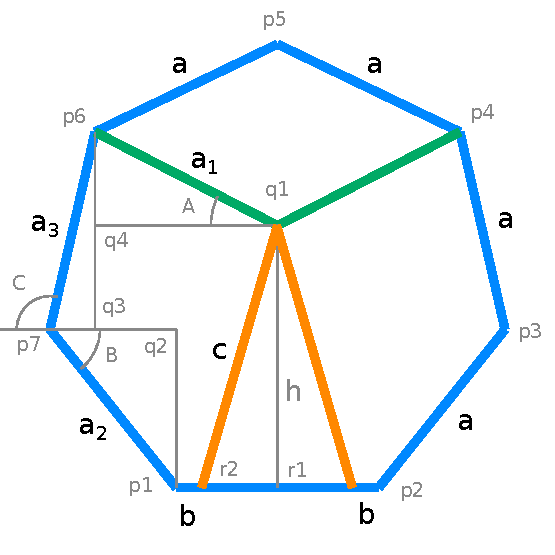
\includegraphics[scale=1]{figs/heptagon_plan.pdf}
\caption{The meccano heptagon is defined with two integers $a > b$. A third value $c$ is checked to be an integer too to form a valid heptagon.}
\label{heptagonplan}
\end{figure}

Consider the heptagon in figure \ref{heptagonplan}.
First start with the three angles $A$, $B$ and $C$:

\begin{align*}
A &= {\pi/7} \\
B &= {2\pi/7} \\
C &= {3\pi/7} \\
\end{align*}

Then find the sines, nothing that the regular heptagon side is $a = a_1 = a_2 = a_3$:

\begin{align*}
sin(A) &= \frac{\overline{q_4 p_6}}{a_1} \\
sin(B) &= \frac{\overline{p_1 q_2}}{a_2} \\
sin(C) &= \frac{\overline{p_6 q_3}}{a_3} \\
\end{align*}

From the figure the height $h$ corresponds to:

\begin{align*}
h &= \overline{p_1 q_2} + \overline{p_6 q_3} + \overline{p_6 q_4} \\
  &= a(sin(A) + sin(B) + sin(C))
\end{align*}

According to \url{https://en.wikipedia.org/wiki/Heptagonal_triangle}

\begin{align*}
sin(A) + sin(B) + sin(C) &= -\frac{\sqrt{7}}{2}
\end{align*}

So

\begin{align*}
h &= \frac{\sqrt{7}a}{2}
\end{align*}

Finally we get the $c$ length as a function of lengths $a$ and $b$:

\begin{align*}
c^2 &= \overline{r_1 r_2}^2 + h^2 \\
    &= \frac{(a - b)^2}{4} + \frac{7a^2}{4} \\
    &= \frac{8a^2 - 2ab + b^2}{4}
\end{align*}

\begin{figure}[htp]
\centering
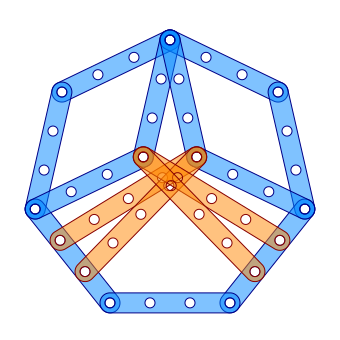
\includegraphics[scale=1]{figs/heptagon-3}
\caption{The first meccano heptagon with values $a=3$, $b=1$ and $c=4$.}
\label{heptagon-3}
\end{figure}

\begin{figure}[htp]
\centering
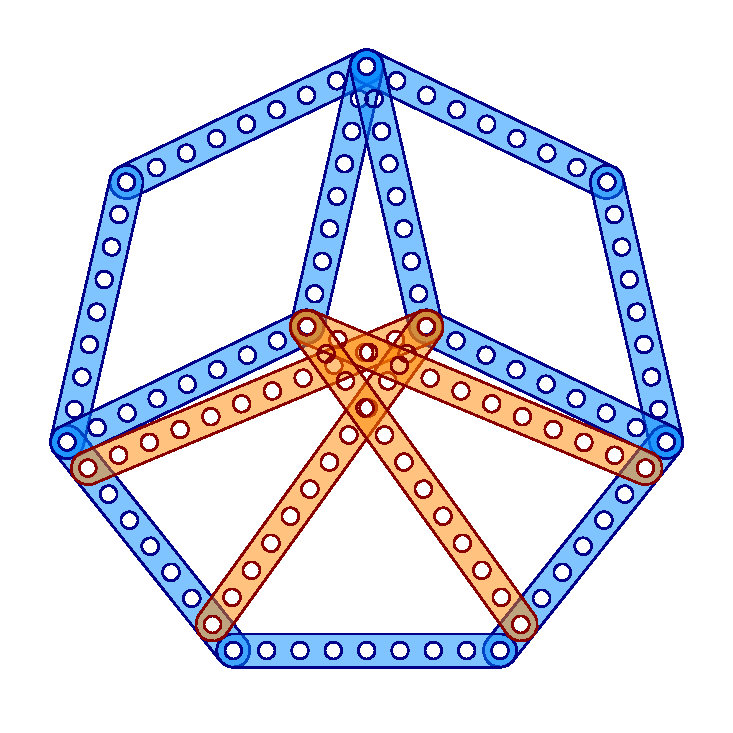
\includegraphics[scale=1]{figs/heptagon-8}
\caption{The second meccano heptagon with values $a=8$, $b=1$ and $c=11$.}
\label{heptagon-8}
\end{figure}

A valid meccano heptagon will have the three lenghts $a$, $b$ and $c$ as integers. With a software routine we look for c to be integer by incrementing the values of $a > b$. Figures \ref{heptagon-3} and \ref{heptagon-8} show the first two cases satisfying such condition.




\end{document}

